\documentclass[11pt]{article}
\usepackage{amsmath, amssymb, amsthm}
\usepackage{tikz}
\usetikzlibrary{calc}
\usepackage{eso-pic}
\usepackage{hyperref}
\usepackage{listings}
\usepackage{enumitem}
\usepackage{float}
\usepackage[english]{babel}
\usepackage[utf8x]{inputenc}
\usepackage{graphicx}
\usepackage[colorinlistoftodos]{todonotes}
\usepackage{filecontents}
\usepackage{verbatim}
\usepackage{eurosym}
\usepackage[export]{adjustbox}
\usepackage{geometry}
\usepackage{subcaption}
\usepackage{algorithm}
\usepackage{algorithmic}
\usepackage{xepersian}
\settextfont[]{Niloofar.ttf}

\geometry{margin=1in}

\hypersetup{
  colorlinks, linkcolor=red
}

\AddToShipoutPictureBG{%
\begin{tikzpicture}[overlay,remember picture]
\draw[line width=4pt]
    ($ (current page.north west) + (1cm,-1cm) $)
    rectangle
    ($ (current page.south east) + (-1cm,1cm) $);
\draw[line width=1.5pt]
    ($ (current page.north west) + (1.2cm,-1.2cm) $)
    rectangle
    ($ (current page.south east) + (-1.2cm,1.2cm) $);
\end{tikzpicture}
}

\lstdefinelanguage{Kotlin}{
  morekeywords={abstract,actual,annotation,as,break,by,catch,class,companion,constructor,continue,crossinline,data,delegate,do,dynamic,else,enum,expect,external,false,file,final,finally,for,fun,if,in,inner,infix,init,inline,interface,internal,is,lateinit,object,open,operator,out,override,package,private,protected,public,return,sealed,suspend,super,this,throw,true,try,typealias,val,var,vararg,when,where,while},
  sensitive=true,
  morecomment=[l]{//},
  morecomment=[n]{/*}{*/},
  morestring=[b]",
  morestring=[b]',
  morestring=[b]"""
}

\begin{document}

\begin{titlepage}

\newcommand{\HRule}{\rule{\linewidth}{0.5mm}}

\center 

\textsc{\LARGE به نام خدا}\\[1.5cm] 


\includegraphics[width=0.4\textwidth]{IUSTLogo.png}\\[2cm] 

\textsc{\Large آشنایی با شبکه های تلفن همراه}\\[0.5cm] 

\HRule \\[0.4cm]
{ \huge \bfseries پروژه پایانی}\\[0.4cm] 
\HRule \\[1.5cm]

\begin{minipage}{0.4\textwidth}
\begin{flushright} \large
\emph{دانشجویان:}\\
محمد درمانلو \\
سید مهدی حسینی زاده\\
\end{flushright}
\end{minipage}
~
\begin{minipage}{0.4\textwidth}
\begin{flushright} \large
\emph{استاد درس: } \\
جناب آقای دکتر دیانت  \\
\end{flushright}
\end{minipage}\\[2cm]

{\large مهلت ارسال: 1403/04/15}\\[2cm]
\vfill 
\end{titlepage}

\newpage

\section{مقدمه}
هدف این پروژه توسعه یک نرم‌افزار مبتنی بر Android است که با استفاده از توان دریافتی از سلول‌های شبکه، مکان آن‌ها را تخمین بزند. پروژه به دو بخش اصلی تقسیم می‌شود: تخمین فاصله براساس قدرت سیگنال دریافتی (RSSI) و تخمین مکان سلول‌ها با استفاده از الگوریتم‌های مکان‌یابی هندسی.

\section{بخش اول: تخمین فاصله براساس RSSI}

\subsection{مقدمه}
در این بخش، هدف محاسبه فاصله تخمینی بین دستگاه تلفن همراه و ایستگاه پایه با استفاده از قدرت سیگنال دریافتی (RSSI) است. این محاسبه براساس مدل افت مسیر Path Loss انجام می‌شود.

\subsection{مدل افت مسیر}
مدل افت مسیر شامل سه پارامتر اصلی است:
\begin{itemize}
    \item \textbf{فاصله مرجع (REFERENCE\_DISTANCE)}: فاصله مرجع که معمولاً برابر با 1 متر است.
    \item \textbf{افت مسیر در فاصله مرجع (PATH\_LOSS\_AT\_REFERENCE\_DISTANCE)}: افت مسیر در فاصله مرجع که به دسی‌بل بیان می‌شود و به محیط بستگی دارد.
    \item \textbf{توان افت مسیر (PATH\_LOSS\_EXPONENT)}: توانی که افت مسیر با افزایش فاصله تغییر می‌کند و به محیط بستگی دارد.
\end{itemize}

\subsection{فرمول محاسبه فاصله}
فرمول استفاده شده برای محاسبه فاصله به صورت زیر است:
\[
\text{distance} = \text{REFERENCE\_DISTANCE} \times 10^{\frac{\text{PATH\_LOSS\_AT\_REFERENCE\_DISTANCE} - \text{rssi}}{10 \times \text{PATH\_LOSS\_EXPONENT}}}
\]

در این فرمول:
\begin{itemize}
    \item \text{distance}: فاصله تخمینی (به متر)
    \item \text{rssi}: قدرت سیگنال دریافتی (به dBm)
\end{itemize}

\subsection{کد کاتلین}
کد های کاتلین و جاوا این بخش (قسمت اول) در فایل RssiDistanceCalculator که در مسیر پروژه و فولدر buisiness قرار دارد .

\section{بخش دوم: تخمین مکان سلول‌ها}

\subsection{مقدمه}
در این بخش، هدف تخمین مکان دقیق سلول‌ها با استفاده از فاصله‌های بدست آمده از بخش اول و الگوریتم‌های مکان‌یابی هندسی است. از الگوریتم کمینه مربعات Least Squares برای بهینه‌سازی مکان تخمینی استفاده می‌شود.

\subsection{الگوریتم مکان‌یابی دایره‌ای Circular Lateration}
الگوریتم مکان‌یابی دایره‌ای یکی از روش‌های مرسوم برای تخمین مکان است که براساس فاصله‌های محاسبه شده از چندین گره مرجع انجام می‌شود.

\subsection{مدل ریاضی}
مدل ریاضی الگوریتم مکان‌یابی دایره‌ای شامل معادلاتی است که براساس فاصله‌های بین گره هدف و گره‌های راهنما به دست می‌آید:
\[
(x - x\_i)^2 + (y - y\_i)^2 = d\_i^2
\]
که در آن:
\begin{itemize}
    \item x و  y مختصات مکان تخمینی
    \item x\_i و  y\_i مختصات گره راهنما
    \item d\_i فاصله تخمینی از گره راهنما
\end{itemize}

\subsection{کد کاتلین}
کد کاتلین بخش دوم در فایل CircularLateration که در مسیر پروژه و فولدر buisiness قرار دارد .

\section{گرفتن سلول های گوشی }

بخشی اصلی کد در این فایل قرار دارد استفاده از TelephonyManager (مدیر تلفنی) اطلاعات مربوط به سلول‌های مخابراتی را از دستگاه دریافت می‌کند. این TelephonyManager به برنامه‌نویس اجازه می‌دهد تا به اطلاعات شبکه مخابراتی (مانند سیگنال LTE) دسترسی داشته باشد و از طریق آن می‌تواند اطلاعاتی مانند شدت سیگنال (RSSI) و شناسه سلول Cell ID را بدست آورد.

این بخش از کد (getCellInfo) در حلقه‌ای بی‌نهایت اجرا می‌شود و به طور مداوم اطلاعات را از تلفن همراه خوانده و ثبت می‌کند. به طور خاص، این بخش:

مجوزهای لازم را بررسی می‌کند تا اطمینان حاصل کند که اجازه دسترسی به موقعیت جغرافیایی و دیگر داده‌های مورد نیاز در دسترس است.

اطلاعات مکان فعلی دستگاه را از متغیر deviceX و deviceY بدست می‌آورد که به صورت جفتی از عدد اعشاری (Double) مختصات عرض و طول جغرافیایی را نشان می‌دهند.

از telephonyManager.allCellInfo استفاده می‌کند تا اطلاعات مختلفی مانند rssi (شدت سیگنال دریافتی) و فاصله محاسبه‌شده (distance) را از هر سلول LTE دریافت کند.

اطلاعات دریافت شده را به صورت ReceivedSignalEntity (شامل شناسه سلول، مختصات دستگاه، فاصله و شدت سیگنال) ثبت می‌کند و این اطلاعات را به کمک mainRepository (که مسئول دسترسی به داده‌های برنامه و ذخیره‌سازی است) ذخیره می‌کند.

در نهایت، با تأخیر 10 ثانیه مجدداً اطلاعات را بررسی و ثبت می‌کند، تا اطلاعات به روز شده و در سیستم ذخیره شوند.

این کد مجموعه‌ای از عملکردها و متدهای بکار گرفته شده در ViewModel است که به منظور مدیریت و ذخیره داده‌ها از طریق mainRepository اجرا می‌شود و تمرکز اصلی آن بر روی دریافت و پردازش اطلاعات از شبکه‌های مخابراتی و مکان‌یابی است.

\section{روند اجرای برنامه }
بطور کلی روند اجرای برنامه به شرح زیر است:
\subsection{گرفتن اطلاعات مربوط به سلول ها}
در فاصله های زمانی ۱۰ ثانیه ای‌ با استفاده از سرویس TelephonyManager، اطلاعات مربوط به سلول هایی از شبکه که گوشی کاربر با آن ها ارتباط دارد گرفته می شوند. این اطلاعات شامل cell id, rssi, mnc,, mcc و ... است.
\subsection{فاصله تقریبی}
در مرحله بعد با استفاده از مدل Path Loss و rssi سلول، فاصله تقریبی سلول از گوشی کاربر تخمین زده می شود
این اندازه گیری باید به دفعات متعدد (حداقل ۳) و در مکان های مختلفی انجام شود.
\subsection{پیدا کردن مختصات تقریبی}
در مرحله پایانی با استفاده از الگوریتم CircularLateration و فاصله های تخمین زده شده، مختصات تقریبی سلول مورد نظر را تخمین می زنیم.

\section{صفحات پروژه}
اپلیکیشن از دو صفحه تشکیل می شود:
\subsection{صفحه logs}
در صفحه Logs، گزارش مربوط به اطلاعات سلول هایی دریافتی را به همراه زمان گزارش مشاهده می کنیم.
\subsection{صفحه Positioned Cells}
در صفحه Positioned Cells, اطلاعات مربوط به همه ی سلول هایی که گوشی کاربر با آنها ارتباط گرفته و دیتای لازم برای محاسبه مختصات آنها وجود داشته است را مشاهده می کنیم.
اطلاعات موجود در این صفحات هر ۱۰ ثانیه آپدیت خواهند شد.

\begin{figure}[htbp]
    \centering
    \begin{minipage}[b]{0.45\textwidth}
        \centering
        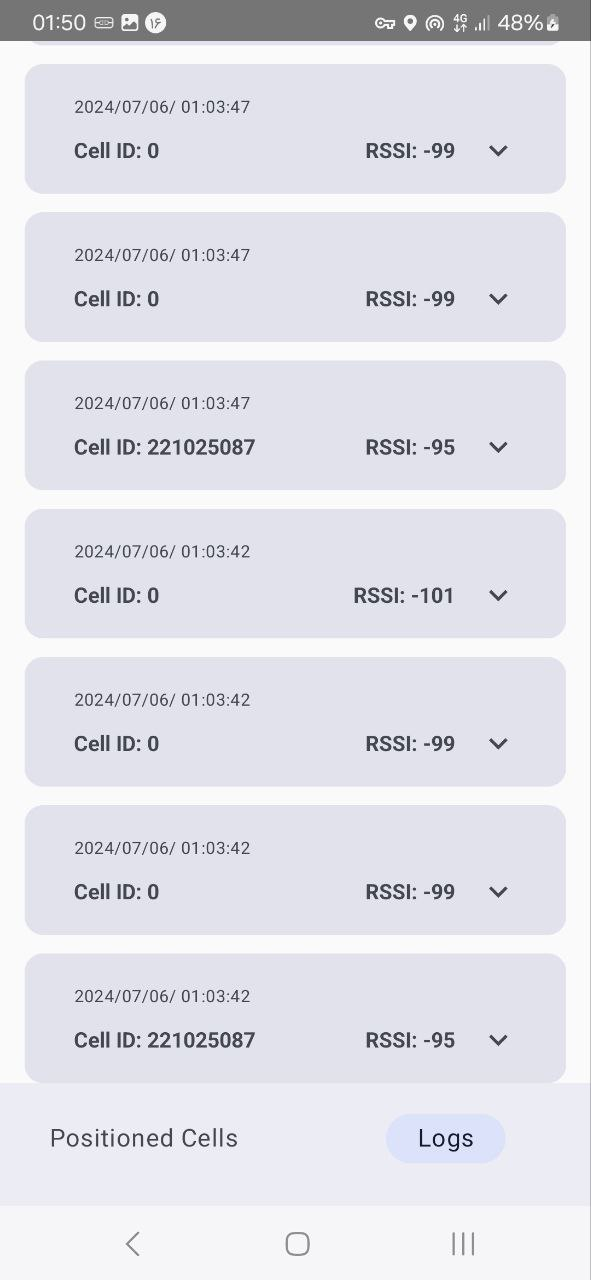
\includegraphics[width=\textwidth]{Output1.jpg}
        \caption{عکس از صفحه Logs}
    \end{minipage}
    \hfill
    \begin{minipage}[b]{0.45\textwidth}
        \centering
        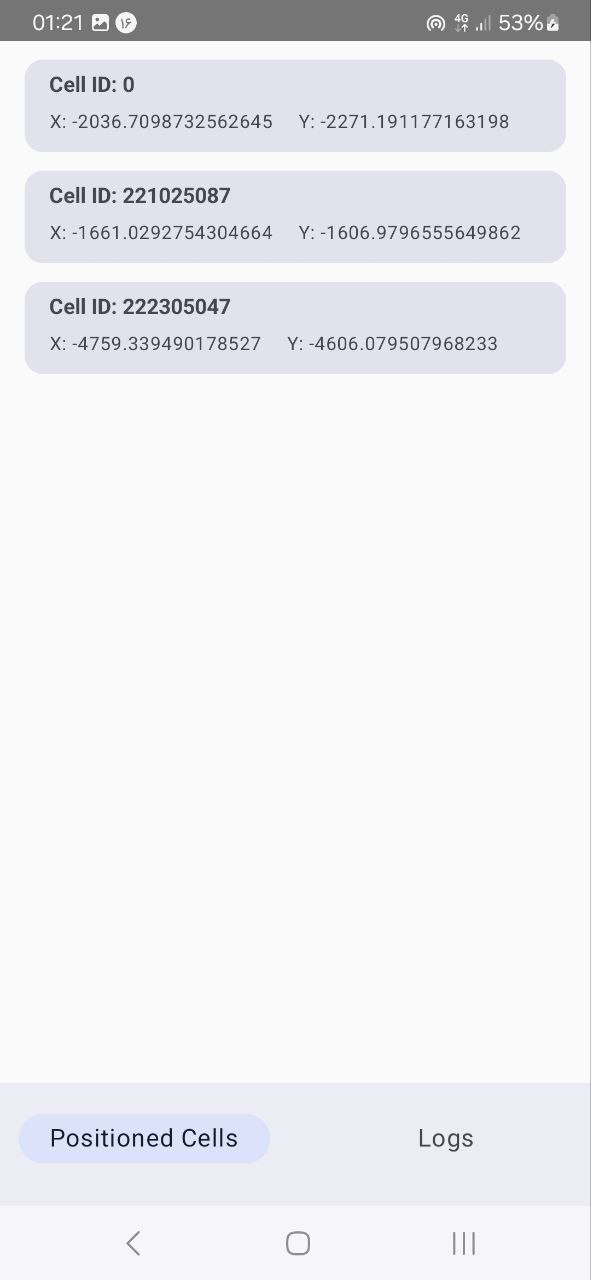
\includegraphics[width=\textwidth]{Output2.jpg}
        \caption{عکس از صفحه Cell Positions}
    \end{minipage}
\end{figure}



\end{document}